% !TEX root = pa_doc.tex
\begin{markdown}

% TODO: rename file

# Architecture

*add image*

## Frontend
For the presentation of the web application to the user, we used React\cite{React}. We decided to use React because of its potential to write cleaner code with component based modularity. To minimise potential problems and to insure a a unidirectional data flow we chose to incorporate  the flux pattern into the architecture design, instead of using the typical Model View Controller (MVC) architecture.

The data for the front end is provided by the back end RESTful API service and retrievable through HTTP calls. Each fetch request is cached using a service worker. We built the service worker using Workbox\cite{Workbox}. Workbox is a library that implements in a set of service worker best practices and helps you get the most out of your service workers.

### PWA
\say{Progressive Web Apps (PWA) are experiences that combine the best of the web and the best of apps.}\cite{WhatIsPWA}

Google and other companies have developed a new, modern web application standard. PWAs implement said standard and receive additional permission as a rewarded for doing so. This allows PWA to behave and feel like native apps. They live can on the user's home screen, offer a full screen experience, access device hardware (camera, GPS, etc) and can even re-engage users with push notifications\cite{PWA}.  When launched from the user’s home screen a Progressive Web App can load instantly, regardless of the network state. This is done by with the help of service workers.

#### Service Workers
A service worker is like a client-side proxy and that allows control of the cache. You can improve the loading speed of your page by pre-caching key resources. Using cache also eliminates the dependence on the network, ensuring a reliable offline experience for your users.\cite{ServiceWorker}

### React
React\cite{React} was originaly developed by Facebook and is one of the most popular UI librarys. It allows you to create reusable Compents using JSX, a syntax extension to JavaScript.
The idea behind React is to design simple views for each state of the application. Doing so allows it to only update and render components that need to be changed, thereby improving performance immensely.

#### Flux
Flux\cite{OurReadme} is a application pattern developed by Facebook. It's goal is to insure a a unidirectional data flow in React apps. The use of this practice enhances the quality and performance of the code by improving the data consistency. It is the optimal architecture for the use of React.

\begin{figure}[H]
  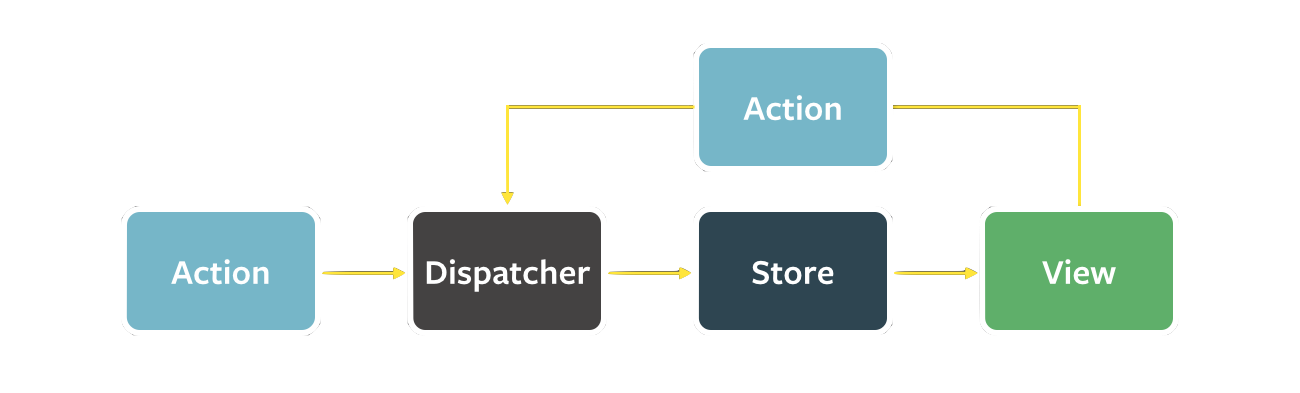
\includegraphics[width=10cm, center]{./assets/flux.png}
  \caption{Flux Model{\cite{FluxModel}}}
\end{figure}



% TODO: bild ref https://facebook.github.io/flux/img/flux-simple-f8-diagram-with-client-action-1300w.png

In Flux, the dispatcher is a singleton that directs the flow of data to ensure that updates do not cascade, which would lead to unpredictable behaviour. When a user interacts with a React view, the view sends an action through the dispatcher, which notifies the stores that hold the application’s data. When the stores change state, the view gets notified and changes accordingly.


## Backend
The Sever-side of ZHAWo is implemented in NodeJS\cite{Node}. We use the ExpressJS Server to handle all the API calls.

### NodeJS
Node.js is a JavaScript runtime environment, designed to build scalable network applications\cite{Node}.
*öpis vo da https://nodejs.org/en/about/* blocking and so on
#### Express
Express\cite{Express} is a minimal and flexible web application framework for Node.js. It provides HTTP utility methods and allows you to create a robust API.

% TODO: add image front-back api calls and stuff



\end{markdown}
